\documentclass[graybox]{svmult}

\usepackage[utf8]{inputenc}
\usepackage{makeidx}
\usepackage{graphicx}
\usepackage{multicol}
\usepackage[bottom]{footmisc}
\usepackage{newtxtext}
\usepackage{newtxmath}
\RequirePackage[l2tabu, orthodox]{nag}

% Allow PDF 1.7 documents to be used in \includegraphics
\pdfminorversion=7

\graphicspath{{./img/}}

\makeindex

\begin{document}

\title*{An MPI Framework for HPC Clusters Deployed with Software-Defined
Networking}
% Use \titlerunning{Short Title} for an abbreviated version of
% your contribution title if the original one is too long
\author{Keichi Takahashi, Susumu Date, Yasuhiro Watashiba, Yoshiyuki Kido,
Shinji Shimojo}
% Use \authorrunning{Short Title} for an abbreviated version of
% your contribution title if the original one is too long
\institute{Keichi Takahashi \at Nara Institute of Science and Technology,
8916-5 Takayama, Ikoma, Nara, Japan\\ \email{keichi@is.naist.jp}
\and Susumu Date, Yasuhiro Watashiba, Yoshiyuki Kido, Shinji Shimojo \at
Cybermedia Center, Osaka University, 5-1 Mihogaoka, Ibaraki, Osaka, Japan\\
\email{\{date, watashiba-y, kido, shimojo\}@cmc.osaka-u.ac.jp}}
%
% Use the package "url.sty" to avoid
% problems with special characters
% used in your e-mail or web address
%
\maketitle

\abstract*{Each chapter should be preceded by an abstract (no more than 200
words) that summarizes the content. The abstract will appear \textit{online}
at \url{www.SpringerLink.com} and be available with unrestricted access. This
allows unregistered users to read the abstract as a teaser for the complete
chapter. Please use the 'starred' version of the \texttt{abstract} command for
typesetting the text of the online abstracts (cf. source file of this chapter
template \texttt{abstract}) and include them with the source files of your
manuscript. Use the plain \texttt{abstract} command if the abstract is also to
appear in the printed version of the book.}

\abstract{Each chapter should be preceded by an abstract (no more than 200
words) that summarizes the content. The abstract will appear \textit{online}
at \url{www.SpringerLink.com} and be available with unrestricted access. This
allows unregistered users to read the abstract as a teaser for the complete
chapter.\newline\indent Please use the 'starred' version of the
\texttt{abstract} command for typesetting the text of the online abstracts
(cf. source file of this chapter template \texttt{abstract}) and include them
with the source files of your manuscript. Use the plain \texttt{abstract}
command if the abstract is also to appear in the printed version of the book.}

\section{Introduction}

Lorem Ipsum is simply dummy text of the printing and typesetting industry.
Lorem Ipsum has been the industry's standard dummy text ever since the 1500s,
when an unknown printer took a galley of type and scrambled it to make a type
specimen book. It has survived not only five centuries, but also the leap into
electronic typesetting, remaining essentially unchanged. It was popularised in
the 1960s with the release of Letraset sheets containing Lorem Ipsum passages,
and more recently with desktop publishing software like Aldus PageMaker
including versions of Lorem Ipsum~\cite{Takahashi2014}. including versions of
Lorem Ipsum~\cite{Takahashi2015}. including versions of Lorem
Ipsum~\cite{Takahashi2017}. including versions of Lorem
Ipsum~\cite{Takahashi2018}. including versions of Lorem
Ipsum~\cite{Dashdavaa2014}.


\section{Problem}

\begin{figure}
    \centering
    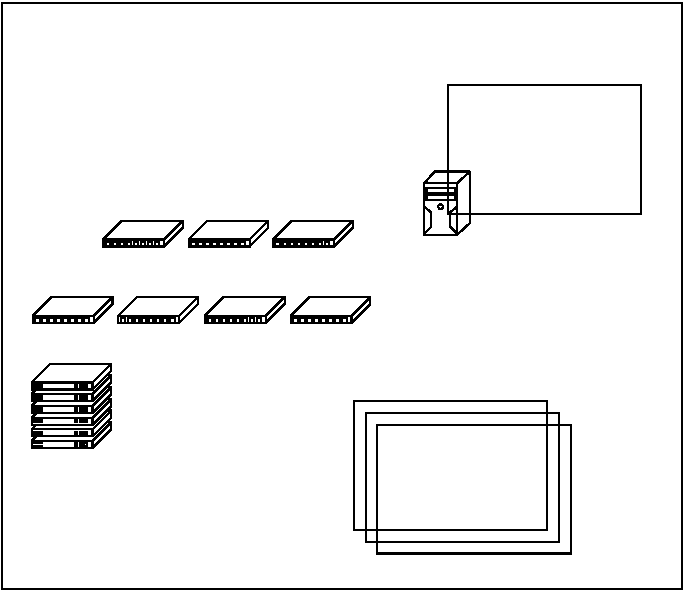
\includegraphics{arch}
    \caption{Performance Development of Top500 HPC Systems}%
    \label{kt:fig:top500-rmax}
\end{figure}

\section{Proposal}

\section{Preliminary Evaluation}

\section{Conclusion}

\bibliographystyle{spmpsci}
\bibliography{references}

\end{document}
